%    \begin{macrocode}
\documentclass[digital,nocover,nolot]{fithesis3}
\usepackage[english]{babel}
\usepackage{hologo}
\usepackage{fancyvrb}
\usepackage{minted}
\usepackage{ltxcmds}
\usepackage{tabularx}
\makeatletter
\thesissetup{
  title=A fithesis3 user guide for the \thesis@english@facultyName,
  TeXtitle=A \textit{fithesis3} user guide\medskip\\\Large for the
    \thesis@english@facultyName,
  type=bc,
  department=Department of Computer Graphics and Design,
  programme=Applied Informatics,
  field=Typesetting,
  titleEn=\thesis@title,
  departmentEn=\thesis@department,
  programmeEn=\thesis@programme,
  fieldEn=\thesis@field,
  author=Vít Novotný,
  advisor={Doc.\ RNDr.\ Petr Sojka, Ph.D.},
  assignment={},
  keywords={thesis, typesetting, LaTeX},
  TeXkeywords={thesis, typesetting, \LaTeX{}},
  keywordsEn=\thesis@keywords,
  TeXkeywordsEn=\thesis@TeXkeywords,
  abstractEn=\thesis@abstract,
  faculty=\jobname,
  bib=guide.bib,
  autoLayout=false}
\thesislong{abstract}{%
  \textsf{Fithesis3} is a \LaTeX{} document class, which
  streamlines the typesetting of the mandatory parts of theses, so
  that the author can focus at content alone. \textsf{Fithesis3}
  can be used to write theses in various languages across the
  faculties of the \thesis@english@universityName.

  This document describes the installation of the
  \textsf{fithesis3} class, its configuration and its use at the
  \thesis@english@facultyName. As a demonstration of its
  capabilities, this document was typeset using the
  \textsf{fithesis3} class.}
\makeatother
\thesisload% The menukeys package does not play nice, when it is
  \usepackage[os=win]{menukeys}% loaded before BibLaTeX.
\begin{document}
  \makeatletter\thesis@preamble\makeatother
  \chapter{Introduction}
  To use the \textsf{fithesis3} class, you can use an online
  \LaTeX{} editor, such as Overleaf%
  \footnote{Overleaf \textsf{fithesis3}
%<*sci>
    and \textsf{sci.muni.thesis}
%</sci>
    templates are located at
    \url{http://www.overleaf.com/gallery/tagged/muni}.},
  which allows you to skip the installation described in Section
  \ref{sec:install} completely.
%<*sci>
  Beside \textsf{fithesis3}, the \textsf{sci.muni.thesis} \LaTeX\
  package, as well as templates for common word processors, can
  likewise be used for the preparation of theses at the
  \makeatletter\thesis@english@facultyName\makeatother\footnote{%
    For more information about the alternative templates, see
    \url{http://www.sci.muni.cz/cz/BcMgrStudium/Legislativa/Sablony}.}.
%</sci>
  
%<*fi>
  {\makeatletter\newcount\thguide@tl\expandafter\thguide@tl\the
  \year\if\month<7\advance\thguide@tl-1\fi\makeatother
  Another way to avoid installation is to use any public-access
  computer at the \makeatletter\thesis@english@facultyName
  \makeatother\ that runs Microsoft Windows. By running
  \begin{center}
    \makeatletter\menu[,]{Start,Programs,Document Tools,TeXLive%
    \the\thguide@tl\ namapovani na T}\makeatother
  \end{center} you can mount the faculty \TeX\ Live installation to
  drive \verb'T:\'. Consequently, you can either use the command
  line to run commands from the \TeX{} distribution by running
  \begin{center}
    \makeatletter\menu[,]{Start,Programs,Document Tools,TeXLive%
    \the\thguide@tl\ CMD}\makeatother
  \end{center}
  or you can use the graphical \TeX\ editor \TeX Works by running
  \begin{center}
    \makeatletter\menu[,]{Start,Programs,Document Tools,TeXWorks+%
    TeXLive\the\thguide@tl}\makeatother
  \end{center}}

  Yet another way to avoid installation is to either connect to the
  Linux server at \url{aisa.fi.muni.cz} over SSH, or use any
  public-access computer at the
  \makeatletter\thesis@english@facultyName\makeatother\ that runs
  Linux or Mac OS, and load the faculty \TeX\ Live installation by
  issuing the \texttt{module add texlive} command on the command
  line. If you choose this approach, you can also skip the entire
  Section \ref{sec:install}, although a certain degree of
  proficiency in working with a Unix operating system is required
  compared to the other methods.
%</fi>
  \makeatletter
    % This macro kerns an icon next to a word.
    \def\thguide@iconkern{\kern.2ex}
  \makeatother
%<*sci>
  \makeatletter
    % This macro typesets the URL of a math.muni server.
    \def\thguide@server#1{%
      \includegraphics[height=.5em]{resources/#1.pdf}%
      \thguide@iconkern\url{#1.math.muni.cz}}
  \makeatother
  Another way to avoid installation is to use the faculty \TeX\ Live
  installation by connecting to the Linux server at
  \makeatletter\thguide@server{yoda}\makeatother\ or
  \makeatletter\thguide@server{vader}\makeatother\ over SSH
  (through port 22222) or over the remote desktop
  protocol\footnote{
    For more information about connecting through the remote
    desktop protocol, see
    \url{http://www.math.muni.cz/aktuality/347-vzdaleny-pristup-yoda-vader.html}.}
  (through port 13556), or to use any public-access computer at the
  \makeatletter\thesis@english@facultyName\makeatother\ that runs
  Linux. If you choose this approach, you can also skip this entire
  section, although a certain degree of proficiency in working with
  a Unix operating system is required compared to the first method.
%</sci>
  
  \section{Installation}\label{sec:install}
  \subsection{Installing a \TeX{} distribution}
  If you decided not to use a public \TeX{} distribution, you will
  need to install one locally before proceeding further. A \TeX{}
  distribution contains tools and packages that are going to help
  you with preparing and typesetting your \LaTeX\ documents.

  The two major \TeX{} distributions that you can install are
  Mik\TeX\footnote{Mik\TeX\ can be acquired from
  \url{http://miktex.org/2.9/setup}.}, which can be used with the
  Microsoft Windows operating system, and \TeX\ Live\footnote{%
  \TeX\ Live can be acquired from
  \url{http://www.tug.org/texlive}.}, which can be installed on
  both Unix and Windows operating systems. The advantages of
  Mik\TeX\ over \TeX Live include refined graphical user interface
  and the ability to install new packages on the fly.
  
  Along with Mik\TeX{}, you will also need to install a Perl
  interpreter, such as Strawberry Perl\footnote{Strawberry Perl can
  be downloaded from \url{http://strawberryperl.com/}.}. \TeX\ Live
  installs a Perl interpreter by default.

  \subsection{Installing packages}\label{sec:req-packages}
  In order to function properly, \textsf{fithesis3} needs the
  following packages packages to be installed in your \TeX\
  distribution: \textsf{keyval}, \textsf{etoolbox},
  \textsf{ifxetex}, \textsf{ifluatex}, \textsf{inputenc},
  \textsf{xcolor}, \textsf{graphix}, \textsf{pdfpages},
  \textsf{hyperref}, \textsf{microtype}%
  {\makeatletter
  % This macro typesets loaded packages.
  \def\thguide@prnpkg#1{\ltx@ifpackageloaded
    {#1}{, \textsf{#1}}{}}%
  \thguide@prnpkg{tikz}%
  \thguide@prnpkg{changepage}%
  \thguide@prnpkg{setspace}%
  \thguide@prnpkg{geometry}},
  \textsf{fontspec}, \textsf{unicode-math}, \textsf{mathpazo},
  \textsf{tex-gyre-pagella}, \textsf{lm}, \textsf{cmap},
  \textsf{fontenc}, \textsf{tabularx}, \textsf{tabu},
  \textsf{booktabs}, \textsf{csquotes}, \textsf{biblatex},
  \textsf{fithesis}.
 
  {\makeatletter %% A placeholder string macro
  \def\thguide@placeholder#1{$\langle$\textit{#1}$\rangle$}
  If you performed a full installation of \TeX\ Live, you should
  already have all the required packages installed. If you are
  using a partial installation of \TeX\ Live, you can use the
  \texttt{tlmgr} command-line tool by executing \texttt{tlmgr
  install} \thguide@placeholder{pkgname}, where
  \thguide@placeholder{pkgname} is the name of the package you wish
  to install. In some cases, \TeX\ Live may assign a different name
  to a package. To find out the \TeX\ Live name of a package, open
  the
  \texttt{http://www.ctan.org/pkg/}\thguide@placeholder{pkgname}
  webpage in a web browser. It should contain the following text:
  \begin{center}
    Contained in \TeX\ Live as \thguide@placeholder{texlivename}
  \end{center}
  where \thguide@placeholder{texlivename} corresponds to the \TeX\
  Live name of the package. Use this name instead of
  \thguide@placeholder{pkgname} with \texttt{tlmgr}.
  Alternatively, you can download the packages manually from
  \texttt{http://www.ctan.org\discretionary{/}{/}{/}pkg/}%
  \thguide@placeholder{pkgname} and extract them into the
  \texttt{texmf/} directory located in your user home directory.
  Mind that the packages themselves may depend on other
  packages; if you are using a partial installation of \TeX\ Live,
  you will have to resolve these dependencies manually by
  inspecting the documentation of each package.

  If you use Mik\TeX\ and you enabled the \textit{over the air
  installation of packages} during the installation, Mik\TeX\ will
  automatically download all the required packages, when you first
  typeset a \textsf{fibeamer} document. If you didn't enable this
  feature, you will need to enter the Mik\TeX\ package manager by
  running
  \begin{center}
    \menu[,]{Start,MikTeX,MikTeX Package Manager (Admin)}
  \end{center}
  and download the packages manually through the user interface.
  In some cases, Mik\TeX\ may assign a different name to a
  package. To find out the Mik\TeX\ name of a package, open the
  \texttt{http://www.ctan.org\discretionary{/}{/}{/}pkg/}%
  \thguide@placeholder{pkgname} webpage in a web browser,
  where \thguide@placeholder{pkgname} is the name of the
  package you wish to install. It should contain the following
  text:
  \begin{center}
    Contained in Mik\TeX\ as \thguide@placeholder{miktexname}
  \end{center}
  where \thguide@placeholder{miktexname} corresponds to the
  Mik\TeX\ name of the package. If you still can't find the
  package, try synchronizing the package database by selecting 
  \begin{center}
    \menu[,]{Repository,Synchronize}
  \end{center}
  from the menu bar of the Mik\TeX\ package manager. Mind that the
  packages themselves may depend on other packages; if you disabled
  the over the air installation of packages, you will have to
  resolve these dependencies manually by inspecting the
  documentation of each package.}
  
  If you wish to use a newer version of \textsf{fithesis3} than the
  one that is available in your \TeX\ distribution, you should
  download a file named \texttt{fithesis.tds.zip} containing the
  version of the package you wish to use and place it in a root
  directory that is recognized by your \TeX\ distribution. In
  \TeX\ Live\footnote{For more information about the \TeX\ Live root
  directories, see
  \url{http://www.tug.org/texlive/doc/texlive-en/texlive-en.html\#x1-110002.3},
  Chapter 2.3.}, one of such directories is the \texttt{texmf/}
  folder in your user home directory. In Mik\TeX\footnote{
  For more information about the \TeX\ Live root
  directories, see 
  \url{http://docs.miktex.org/manual/localadditions.html}.},
  the list of recognized root directories can be gleaned by
  running
  \begin{center}
    \menu[,]{Start,MikTeX,MikTeX Options (Admin),Roots}
  \end{center}

  \section{Picking a \TeX\ engine}
  There are several programs, called \TeX\ engines, that you can
  use to typeset \textsf{fithesis3} \LaTeX{} source files into
  displayable PDF documents. The ones we will discuss are
  \hologo{pdfTeX} and \Hologo{LuaTeX}.
  
  \Hologo{pdfTeX} is the more conservative choice and most \TeX\
  editors use \hologo{pdfTeX} as the default \TeX\ engine. The main
  advantage \Hologo{LuaTeX} over \hologo{pdfTeX} for a
  \textsf{fithesis3} user is the ability to use standard OpenType
  and TrueType fonts installed on your system, whereas
  \hologo{pdfTeX} is confined to the fonts installed in your \TeX\
  distribution.
  
  If the ability to use arbitrary fonts within your documents
  interests you, Chapter 3 of the \textsf{fontspec} package
  manual\footnote{The \textsf{fontspec} package manual is available
  at \url{http://mirrors.ctan.org/macros/latex/contrib/fontspec/fontspec.pdf}.}
  should provide you with the relevant information. If you are
  only going to use the fonts present in the \TeX{} distribution or
  if you do not intend to change the preset \textsf{fithesis3}
  fonts at all, you can safely use \hologo{pdfTeX}, which is
  currently also considerably faster than \Hologo{LuaTeX}.

  \section{Creating and typesetting a \textsf{fithesis3} document}
  Before using the \textsf{fithesis3} class, it is useful to be
  familiar with the \LaTeX{} typesetting system. A good way to get
  started is to read one of the introductory texts in English
  \cite{veryshortlatex,shortlatex,longlatex,latex} or in Czech
  \cite{rybicka03,satrapa11}. Taking one of the \textit{FI:PB029},
  \textit{PřF:M5751}, or \textit{FF:PLIN028} courses taught at
  the \makeatletter\thesis@english@universityName\makeatother\ is
  also helpful.
  
  To become familiar with \textsf{fithesis3}, you are encouraged to
  inspect the example documents \makeatletter
  \texttt{\thesis@faculty-pdflatex.pdf} and
  \texttt{\thesis@faculty-lualatex.pdf} as well as their \LaTeX{}
  source files that are named \texttt{\thesis@faculty-pdflatex.tex}
  and \texttt{\thesis@faculty-lualatex.tex}. The example documents
  are distributed along with the package inside the
  \texttt{example/} directory\footnote{The example
  \textsf{fithesis3} documents are also available online at
  \url{http://mirror.ctan.org/macros/latex/contrib/fithesis/example/mu}.
  To typeset the example documents, you need to download the
  \texttt{example.bib} file as well, as it contains the
  bibliography database used in the examples.}.  By modifying and
  by typesetting these \LaTeX{} source files using either the
  \hologo{pdfTeX} or the \Hologo{LuaTeX} engine, you can quickly
  gain a working knowledge of \LaTeX{} and use these source files
  as the basis for your thesis.
  
  If you are using an online editor, such as Overleaf
  \footnote{Overleaf \textsf{fithesis3} templates are located at
  \url{http://www.overleaf.com/gallery/tagged/muni}.}, \LaTeX{}
  source files will be typeset automatically, as you edit them. The
  \TeX{} engine can be selected inside the
  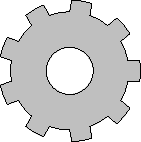
\includegraphics[height=1.3ex]{resources/cog.pdf}\makeatletter
  \thguide@iconkern\makeatother project settings.

  If you are using a graphical \TeX{} editor, such as \TeX
  works\footnote{\TeX works can be downloaded from
  \url{http://www.tug.org/texworks/}.}, you can typeset a \LaTeX{}
  source file by opening the source file from within the editor and
  running either the \hologo{pdfLaTeX} or \Hologo{LuaLaTeX}
  (depending on your choice of \TeX\ engine) command from the task
  bar. The command needs to be executed at least twice to produce
  the table of contents, the list of tables, and the list of
  figures. Additional commands for the typesetting of the
  bibliography and the index are described in the example
  documents.

  If you are using the command line, you can typeset \LaTeX{}
  source files by running either \texttt{pdflatex
  \textit{name.tex}} or \texttt{lualatex
  \textit{name.tex}} (depending on your choice of \TeX\
  engine), where \texttt{\textit{name.tex}} corresponds to the name
  of a \LaTeX\ source file. In the case of the two aforementioned
  example files, the corresponding commands would be:
  \begin{center}\makeatletter
  \texttt{pdflatex \thesis@faculty-pdflatex.tex}
\\\texttt{lualatex \thesis@faculty-lualatex.tex}
  \makeatother\end{center}
  The command needs to be executed from within the directory, where
  the \LaTeX\ source file is located. In Windows, the command line
  can be opened in a directory by holding down the \keys{Shift} key
  and by clicking the right mouse button while hovering the cursor
  over a directory. Select the \menu{Open Command Window Here}
  option in the context menu that opens shortly afterwards.  The
  command also needs to be executed at least twice.

  Beside Overleaf and \TeX works, any text editor can be used to
  modify \LaTeX{} source files. However, it is important to ensure
  that the text editor saves the \LaTeX{} source files in the UTF-8
  text encoding. A \LaTeX{} file saved in a different text encoding
  is likely to be either impossible to typeset or to produce
  unexpected output.

  \chapter{Configuration}
  This chapter provides a full list of the settings that can be
  used to set up and customize the \textsf{fithesis3} class.

  \section{Setting the class options}
  At the beginning of a \textsf{fithesis3} \LaTeX{} source file,
  the command
  \begin{minted}{latex}
\documentclass[option1, option2, ..., optionN]{fithesis3}
  \end{minted}
  is used. The following list summarizes the options that are
  supported by the \textsf{fithesis3} class and their meaning.
  Options that are enabled by default are
  {\makeatletter
  % This macro formats a default class option.
  \def\thguide@default{\itshape}%
  % This macro formats a class option.
  \let\thguide@itemfmt\textbf
  % This macro formats a default printed option.
  \def\thguide@printed{\color{blue}}%
  % This macro formats a default digital option.
  \def\thguide@digital{\color{red}}%
  \thguide@itemfmt{\thguide@default set in italics}.
  \begin{description}
    \item[digital] This option sets the options that are the
      default for the digital version of a thesis. These options
      are \thguide@itemfmt{\thguide@default \thguide@digital set in
      red}.
    \item[\thguide@default printed] This option sets the options
      that are the default for the printed version of a thesis.
      These options are \thguide@itemfmt{\thguide@default
      \thguide@printed set in blue}.
    \item[10pt, 11pt, \thguide@default12pt]
      These options set the font size of the main text to either
      10\,pt, 11\,pt, or 12\,pt, respectively. Using the 12\,pt
      font size with the preset fonts
%<*fi,fsps,fss,law,ped,phil,sci>
      should result in the optimal line width of approximately 66
      characters in one-column typesetting. With two-column
      typesetting, the 10\,pt font size is a better choice,
      yielding approximately the optimal 45 characters per line.
%</fi,fsps,fss,law,ped,phil,sci>
%<*econ,med>
      results in the excessive line width of approximately 86
      characters, which wears the eye of the reader, but is
      required by the page geometry specified by the formal
      requirements of the \thesis@english@facultyName. With
      two-column typesetting, the 11\,pt font size yields
      approximately the optimal 45 characters per line.
%</econ,med>
    \item[oneside]
      This option enables one-sided typesetting. One-sided
      typesetting and printing is generally discouraged. Use only
      if you don't have access to a double-sided printer, or if
      one-sided typesetting is a formal requirement at your
      faculty.
    \item[\thguide@default twoside]
      This option enables double-sided typesetting. Double-sided
      typesetting is generally regarded as more visually pleasing
      and double-sided printing consumes less paper. Use at least
      120 grams per square meter paper to prevent show-through.
    \item[\thguide@default onecolumn]
      This option causes the main text of the thesis to be set in
      one column.
    \item[twocolumn]
      This option causes the main text of the thesis to be set in
      two columns. The two-column format is unconventional in
      theses%
%<*econ,med>
      , although it is more readable and uses the page more
      effectively in the case of the \thesis@english@facultyName
%</econ,med>
      ; you should consult its use with your thesis advisor. If you
      decide to use the two-column format, remember that you also
      need to change the font size option (\thguide@itemfmt{10pt},
      \thguide@itemfmt{11pt}, \thguide@itemfmt{12pt}).
    \item[draft]
      This option replaces any images with blank rectangles and
      marks all overfull lines with black boxes. Other packages
      that you use may behave differently\footnote{
        For more information about the effects of the draft option
        on various packages, see
        \url{http://tex.stackexchange.com/a/49369/70941}.
      } with the \thguide@itemfmt{draft} option specified. This can
      be useful, if you are going to print and proofread a draft of
      your document.
    \item[\thguide@default final]
      Unlike the \thguide@itemfmt{draft} option, this option
      typesets the release version of the document.
    \item[\thguide@default palatino]
      This option sets the roman text font family and the
      mathematical font family to Palatino.
    \item[nopalatino]
      This option prevents \textsf{fithesis3} from setting up the
      fonts. The user must set the fonts manually in the preamble
      of the document.
%<*fi>

      The \thesis@english@facultyName\ has licensed the Comenia
      font family. If you wish to use it in your thesis, you should
      contact Doc.\ RNDr.\ Petr Sojka, Ph.D.
      
      If you are typesetting your thesis on a public-access
      computer at the \thesis@english@facultyName\ or on the
      \url{aisa.fi.muni.cz} Linux server, you can use the
      commercial Math Time mathematical font family,
%</fi>
%<*sci>

      If you are typesetting your thesis on a public-access
      computer at the \thesis@english@facultyName\ that runs Linux
      or on either the \thguide@server{yoda} or
      \thguide@server{vader} Linux server, you can also use the
      commercial Math Time mathematical font family,
%</sci>
%<*sci,fi> 
      which goes well with the \TeX\ Gyre Termes text font family.
      To use Math Time and \TeX\ Gyre Termes within your thesis,
      the preamble of your document should look as follows:
      \begin{minted}{latex}
\documentclass[nopalatino, ...]{fithesis3}
\usepackage{cmap}
\usepackage[T1]{fontenc}
\usepackage{tgtermes}
\usepackage{mathtime}
%% Here goes the rest of the document.
      \end{minted}
%</sci,fi>
    \item[\thguide@default\thguide@digital color]
      This option enables the use of colors. A colorful version of
      the document is more visually pleasing, but shouldn't be used
      in a printed version, if you don't have access to a color
      printer. Unless you have a compelling reason not to, always
      use this option in the electronic version that you are going
      to publish online.
    \item[\thguide@default\thguide@printed monochrome]
      This option disables colors. Disabling colors is generally
      discouraged, unless you don't have access to a color printer.
      However, due to the prevalence of monochrome printing, this
      option is the default.
    \item[\thguide@default microtype]
      This option sets up microtypographic extensions\footnote{
        For more information about the \TeX\ engine
        microtypographic extensions, see
        \url{http://mirrors.ctan.org/macros/latex/contrib/microtype/microtype.pdf}.
      }, which results in visually more pleasing paragraphs of
      text.
    \item[nomicrotype]
      This option prevents \textsf{fithesis3} from setting up
      microtypographic extensions.
    \item[table]
      This option redefines some of the \LaTeX{} table environments
      (\texttt{tabular}, \texttt{tabularx}, and \texttt{tabu}) to
      use alternating colors for odd and even rows. This option
      only works, if the \thguide@itemfmt{color} option is enabled.
    \item[\thguide@default oldtable]
      This option instructs the style not to redefine any table
      environments.
    \item[\thguide@default lot]
      This option causes the list of tables to be included in the
      front matter of the thesis.
    \item[nolot]
      This option removes the list of tables from the front matter
      of the thesis.
    \item[\thguide@default lof]
      This option causes the list of figures to be included in the
      front matter of the thesis.
    \item[nolof]
      This option removes the list of figures from the front matter
      of the thesis.
    \item[\thguide@default\thguide@digital cover]
      This option instructs the class to typeset the cover of the
      thesis on the first pages of the resulting document. A cover
      should be generally present in the electronic version of the
      document for completeness. The cover should not appear inside
      the printed document and should only serve as a template for
      the text imprinted on the front cover of the thesis cover.
    \item[\thguide@default\thguide@printed nocover]
      This option forbids the typesetting of the thesis cover.
      Use, if you are typesetting the printed version of a thesis
      and you are not going to have a cover made for your thesis.
  \end{description}}

  \section{Filling out the metadata}
  Beside the class options, you can also fill out information about
  your thesis by inserting the command
  \begin{minted}{latex}
\thesissetup{
  key1 = {value1},
  key2 = {value2},
      ...
  keyN = {valueN},
}
  \end{minted}
  into the preamble of your thesis. The following list summarizes
  the keys and values that are recognized by the \textsf{fithesis3}
  class and are meaningful for the \makeatletter
  \thesis@english@facultyName\makeatother.

  {\makeatletter\let\thguide@itemfmt\textbf
  \begin{description}
    \item[title]
      This key can be used to specify the title of the thesis. The
      value will be stored as one of the properties of the output
      PDF file; do not use any \LaTeX\ formatting commands within
      the value.
    \item[TeXtitle]
      This key can be used to specify the title of the thesis. The
      value will be typeset on the title page of the resulting PDF
      document, so you can use \LaTeX\ formatting commands within
      the value. If the value of the key is unspecified, the value
      of the \thguide@itemfmt{title} key will be used instead.
%<*sci,econ>
    \item[titleEn]
      This key can be used to specify the English title of the
      thesis. Do not use any \LaTeX\ formatting commands within
      the value.
%</sci,econ>
%<*econ>
      If you are typesetting your thesis in English, this value
      does not need to be specified.
    \item[TeXtitleEn]
      This key can be used to specify the English title of the
      thesis. The value will be typeset on the title page of the
      resulting PDF document, so you can use \LaTeX\ formatting
      commands within the value. If the value of the key is
      unspecified, the value of the \thguide@itemfmt{titleEn} key
      will be used instead. If you are typesetting your thesis in
      English, this value does not need to be specified.
%</econ>
    \item[author]
      This key can be used to specify the full name of the author.
    \item[keywords]
      This key can be used to specify a list of keywords for your
      thesis. The value will be stored as one of the properties of
      the output PDF file; do not use any \LaTeX\ formatting
      commands within the value.
%<*econ,fi,fss,law,med,ped>
    \item[TeXkeywords]
      This key can be used to specify a list of keywords for your
      thesis. The value will be typeset in the resulting PDF
      document, so you can use \LaTeX\ formatting commands within
      the value. If the value of the key is unspecified, the value
      of the \thguide@itemfmt{keywords} key will be used instead.
%</econ,fi,fss,law,med,ped>
%<*econ,fss,law,med,ped>
    \item[keywordsEn]
      This key can be used to specify a list of English keywords
      for your thesis. Do not use any \LaTeX\ formatting commands
      within the value. If you are typesetting your thesis in
      English, this value does not need to be specified.
    \item[TeXkeywordsEn]
      This key can be used to specify a list of English keywords
      for your thesis. The value will be typeset in the resulting
      PDF document, so you can use \LaTeX\ formatting commands
      within the value. If you are typesetting your thesis in
      English, this value does not need to be specified.
%</econ,fss,law,med,ped>
%<*econ,fi,med,ped,sci>
    \item[advisor]
      This key can be used to specify the full name of the thesis
      advisor.
%</econ,fi,med,ped,sci>
    \item[gender]
      This key can be used to specify the gender of the author. It
      is used to determine the suffixes employed in the Czech and
      Slovak locales. If you are typesetting your document in
      English, you don't need to specify this information. The
      valid values include:
      \begin{description}
        \item[m] Male
        \item[f] Female
      \end{description}
    \item[type]
      This key can be used to specify the type of the thesis. The
      recognized types of theses include:
      \begin{description}
        \item[bc]  Bachelor's thesis
        \item[mgr] Master's thesis
        \item[d]   Doctoral thesis
        \item[r]   Rigorous thesis
      \end{description}
    \item[faculty]
      This key can be used to set the faculty at which the thesis
      is going to be defended. To choose the
      \thesis@english@facultyName, use
      \thguide@itemfmt{\thesis@faculty} as the value.
%<*law,med,ped,phil>
    \item[department]
      This key can be used to specify the name of the department at
      which the thesis is going to be defended.
%</law,med,ped,phil>
%<*phil>
      Specifying \texttt{kisk} as the department name changes the
      output to fit the requirements of the Division of Information
      and Library Studies.
%</phil>
%<*sci>
    \item[departmentEn]
      This key can be used to specify the English name of the
      department at which the thesis is going to be defended.
      If you are typesetting your thesis in English, this value
      does not need to be specified.
    \item[programme]
      This key can be used to specify the name of the author's
      study programme.
    \item[programmeEn]
      This key can be used to specify the English name of the
      author's study programme. If you are typesetting your thesis
      in English, this value does not need to be specified.
%</sci>
%<*econ,fsps,med,phil,sci>
    \item[field]
      This key can be used to specify the name of the author's
      field of study.
%</econ,fsps,med,phil,sci>
%<*sci>
    \item[fieldEn]
      This key can be used to specify the English name of the
      author's field of study.
%</sci>
    \item[date]
      This key can be used to specify the date of the thesis
      submission in the \texttt{YYYY/MM/DD} format, where
      \texttt{YYYY} stands for the full year, \texttt{MM} stands
      for the month, and \texttt{DD} stands for the day of month.
%<*econ,fi,fss,law,sci>
    \item[assignment]
      This key can be used to specify a list of PDF files
      containing the scanned thesis assignment. The list should be
      in the following format:
      \begin{center}
        \texttt{path/to/first/file.pdf, path/to/second/file.pdf,}
        \ldots
      \end{center}
%</econ,fi,fss,law,sci>
    \item[bib]
      This key can be used to specify a list of BIB files
      containing the bibliography databases. The list should be in
      the following format:
      \begin{center}
        \texttt{path/to/first/file.bib, path/to/second/file.bib,}
        \ldots
      \end{center}
      When this key is specified, the \textsf{fithesis3} class will
      also automatically typeset a bibliography section. If you
      want more control over where and how the bibliography is
      typeset, use the
      \mintinline{latex}{\printbibliography[bibintoc]} command.

      When the key is not specified, no bibliography will be
      produced, which provides the opportunity for the advanced user
      to set up their bibliography management manually.
  \end{description}
  Apart from the single-paragraph \mintinline{latex}{\thesissetup}
  command, the following keys can be configured with multiple
  paragraphs of text as the value using the command
  \begin{minted}{latex}
\thesislong{key}{%
  The first paragraph

  The second paragraph
  ...
}
  \end{minted}
  \begin{description}
%<*econ,fi,fss,law,med,ped,sci>
    \item[abstract]
      This key can be used to specify the abstract of the thesis.
%</econ,fi,fss,law,med,ped,sci>
%<*econ,fss,law,med,ped,sci>
    \item[abstractEn]
      This key can be used to specify the English abstract of the
      thesis. If you are typesetting your thesis in English, this
      value does not need to be specified.
%</econ,fss,law,med,ped,sci>
    \item[thanks]
      This key can be used to specify the text of the
      acknowledgement.
    \item[declaration]
      This key can be used to specify the text of the declaration.
      If the value of the key is unspecified, the following text is
      going to be used instead in the English locale:
      ``\emph{\thesis@english@declaration}''
  \end{description}
  The complete list of metadata keys can be found in Section 2.2 of
  the technical documentation of the \textsf{fithesis3} class
  \cite{novotny15}.}

  \chapter{Advanced usage}
  This chapter contains a couple of tips for the advanced user, who
  may wishe to configure the class beyond what the class options
  and the metadata settings offer. An understanding of how the
  main routine of \textsf{fithesis3} works is beneficial. The main
  routine is documented in Section 2.4 of the technical
  documentation of the \textsf{fithesis3} class \cite{novotny15}.

  \section{Throubleshooting option clashes}
  If you need to load a package with a specific set of options and the package
  happens to be required by the \textsf{fithesis3} class, as specified in
  Section \ref{sec:req-packages}, you may experience an option clash error. If
  this problem occurs, prepend
  \mintinline{latex}{\PassOptionsToPackage{options}{package}} before the
  \mintinline{latex}{\documentclass[...]{fithesis3}} command. If you need to
  configure the package, you can do that anywhere after the document preamble.
  If the package needs to be configured within the preamble, you can load the
  \textsf{fithesis3} style files prematurely using the
  \mintinline{latex}{\thesisload} command as follows:
  \begin{minted}{latex}
\documentclass[...]{fithesis3}
%% The preamble
\thesisload
%% Here goes the package configuration.
\begin{document}
  %% The document
\end{document}
  \end{minted}
  Note that only a small portion of the packages loaded by
  \textsf{fithesis3} is loaded with a specific set of options. The
  rest of the packages is \emph{lazy-loaded} (loaded only if the
  user hasn't already loaded them), in which case no clash is
  possible.

  \section{Overriding changes made by style and locale files}
  The \textsf{fithesis3} style files are loaded immediately before
  the beginning of your document and may change values you would
  like to set by yourself, such as the \LaTeX\ \texttt{tocdepth}
  and \texttt{secnumdepth} counters. Locale files are also loaded
  immediately before your document, which prevents you from
  changing locale strings from within the preamble of your
  document.
  
  To overcome this limitation, you can load the style and locale
  files prematurely using the \mintinline{latex}{\thesisload} command
  as follows:
  \begin{minted}{latex}
\documentclass[...]{fithesis3}
%% The preamble
\thesisload
%% Here go your changes.
\begin{document}
  %% The document
\end{document}
  \end{minted}
  Although you can use the \mintinline{latex}{\thesisload} command
  anywhere in the preamble, using the macro before the metadata
  configuration will load the default style and locale files not
  taking into account your faculty and locale settings.
  
  The \mintinline{latex}{\thesisload} command also loads the
  \textsf{hyperref} package, which adds hyperlinks and PDF metadata
  into the resulting PDF document. This package is rather delicate,
  as it needs to be loaded after most other packages. Loading
  additional packages after \mintinline{latex}{\thesisload} may
  therefore cause problems.
  
  \section{Changing the layout}
  If you are unsatisfied with the automatic arrangement of the
  mandatory parts of the thesis, you can disable it using the
  \texttt{autoLayout} metadata key:
  \begin{minted}{latex}
\documentclass[...]{fithesis3}
\thesissetup{
%<*econ>
  faculty=econ,
%</econ>
%<*fi>
  faculty=fi,
%</fi>
%<*fsps>
  faculty=fsps,
%</fsps>
%<*fss>
  faculty=fss,
%</fss>
%<*law>
  faculty=law,
%</law>
%<*med>
  faculty=med,
%</med>
%<*ped>
  faculty=ped,
%</ped>
%<*phil>
  faculty=phil,
%</phil>
%<*sci>
  faculty=sci,
%</sci>
  autoLayout=false}
\begin{document}
  A document which, except for this line,
  is completely empty.
\end{document}
  \end{minted}
  \noindent This results in a document that only consists of the main
  matter of the thesis (see Figure \ref{fig:example02}). You can
  now manually insert the preamble and the postamble:
  \begin{minted}{latex}
\documentclass[...]{fithesis3}
\thesissetup{
%<*econ>
  faculty=econ,
%</econ>
%<*fi>
  faculty=fi,
%</fi>
%<*fsps>
  faculty=fsps,
%</fsps>
%<*fss>
  faculty=fss,
%</fss>
%<*law>
  faculty=law,
%</law>
%<*med>
  faculty=med,
%</med>
%<*ped>
  faculty=ped,
%</ped>
%<*phil>
  faculty=phil,
%</phil>
%<*sci>
  faculty=sci,
%</sci>
  autoLayout=false}
\begin{document}
  \makeatletter\thesis@preamble\makeatother
  A document which once again contains all
  the mandatory parts of a thesis.
  \makeatletter\thesis@postamble\makeatother
\end{document}
  \end{minted}
  \begin{figure}[!bt]
    \centering\makeatletter
    \fbox{\includegraphics[clip,trim=2cm 24.5cm 2cm 4.5cm,%
      width=0.975\textwidth]{resources/empty.pdf}}
    \makeatother
    \caption{A document with disabled \texttt{autoLayout}}
    \label{fig:example02}
  \end{figure}
  We are now back to the original document. Instead of inserting
  the \texttt{\string\th e\-sis\-@pre\-amble} and 
  \texttt{\string\th e\-sis\-@post\-amble} commands into the document,
  we can insert only certain sections at the beginning and at the
  end of the document.
  
  The \texttt{\string\th e\-sis\-@preamble} and
  \texttt{\string\th e\-sis\-@postamble} commands set up the proper
  environment and execute the \texttt{\string
  \th e\-sis\-@blocks\-@preamble} and
  \texttt{\string\th e\-sis\-@blocks\-@postamble} commands. To
  change the layout, it is sufficient to redefine \texttt{\string
  \th e\-sis\-@blocks\-@pre\-amble} and
  \texttt{\string\th e\-sis\-@blocks\-@post\-amble} without changing
  the definition of \texttt{\string\th e\-sis\-@pre\-amble} and
  \texttt{\string\th e\-sis\-@post\-amble}. For the
  \makeatletter\thesis@english@facultyName\makeatother,
  \texttt{\string\th e\-sis\-@blocks\-@preamble} expands to the
  following commands:
  {\makeatletter
    % This macro typesets the meaning of another macro.
    \def\thguide@macromeaning#1{%
      \let\ea\expandafter
      \ea\let\ea\thguide@macro\csname#1\endcsname
      \ea\def\ea\thguide@meaning\ea{\meaning\thguide@macro}%
      \def\thguide@parse##1 ##2{%
        ##1\ifx##2\relax\ea\@gobbletwo\else\\\fi\thguide@parse##2}%
      \begin{verse}%
        \ea\ifx\thguide@macro\relax
          $\langle$\emph{empty}$\rangle$
        \else
          \tt\ea\ea\ea\ea\ea\ea\ea\ea\ea\ea\ea\ea\ea\ea\ea\ea\ea\ea
          \ea\ea\ea\ea\ea\ea\ea\ea\ea\ea\ea\ea\ea\thguide@parse\ea
          \ea\ea\ea\ea\ea\ea\ea\ea\ea\ea\ea\ea\ea\ea\@gobbletwo\ea
          \ea\ea\ea\ea\ea\ea\@gobbletwo\ea\ea\ea\@gobbletwo\ea
          \@gobbletwo\thguide@meaning{} \relax
        \fi
      \end{verse}}
    \thguide@macromeaning{thesis@blocks@preamble} and
    \texttt{\string\th e\-sis\-@blocks\-@post\-amble} 
    expands to the following commands:
    \thguide@macromeaning{thesis@blocks@postamble}
  \makeatother}
  To create a document that only contains the title page at the
  beginning of the document and the list of tables at the end of
  the document, we would use the following code:
  \begin{minted}{latex}
\documentclass[...]{fithesis3}
\thesissetup{
%<*econ>
  faculty=econ,
%</econ>
%<*fi>
  faculty=fi,
%</fi>
%<*fsps>
  faculty=fsps,
%</fsps>
%<*fss>
  faculty=fss,
%</fss>
%<*law>
  faculty=law,
%</law>
%<*med>
  faculty=med,
%</med>
%<*ped>
  faculty=ped,
%</ped>
%<*phil>
  faculty=phil,
%</phil>
%<*sci>
  faculty=sci,
%</sci>
  autoLayout=false}
\begin{document}
  \makeatletter
    \def\thesis@blocks@preamble{\thesis@blocks@titlePage}
    \thesis@preamble
  \makeatother
  A document that only contains the title page and the
  list of tables.
  \makeatletter
    \def\thesis@blocks@postamble{\thesis@blocks@lot}
    \thesis@postamble
  \makeatother
\end{document}
  \end{minted}
  The available blocks are documented in Section 3.6 of the
  technical documentation of the \textsf{fithesis3} class
  \cite{novotny15}.
  
  \section{Replacing the backend}
  {\makeatletter\newcommand\thguide@backend[2][]{#2}
  % This macro typesets the used backend class.
  \def\thguide@@backend{\expandafter\thguide@backend\thesis@backend}
  \let\ea\expandafter
  \textsf{Fithesis3} operates on top of the
  \textsf{\thguide@@backend} class, which defines much of the
  document design. To change the backend class, you need to redefine
  the value of \mintinline{latex}{\thesis@backend} from the default
  value of
  \begin{center}
    \ea\ea\ea\mintinline\ea\ea\ea{\ea\ea\ea l\ea\ea\ea a\ea\ea\ea
    t\ea\ea\ea e\ea\ea\ea x\ea\ea\ea}\ea\ea\ea{\ea\string\thesis@backend}
  \end{center}
  to a different value. This assignment needs to be performed prior
  to the \mintinline{latex}{\documentclass} command. If you wanted
  to change the backend class of \textsf{fithesis3} to the
  KOMA-Script \textsf{screprt} with the \texttt{a4paper} option,
  your document would start as follows:}
  \begin{minted}{latex}
\let\ChapFont\bfseries
\let\PageFont\bfseries
\makeatletter
  \def\thesis@backend{[a4paper]{scrreprt}}
\makeatother
\documentclass[...]{fithesis3}
%% Here goes the rest of the document.
  \end{minted}
  The \mintinline{latex}{\ChapFont} and
  \mintinline{latex}{\PageFont} commands are provided by the
  \textsf{rapport3} class, but not by the \textsf{scrreprt} class,
  which is why we needed to define them manually. Inconsistencies
  between different backend classes need to be resolved on a
  case-by-case basis.

  \makeatletter\thesis@postamble\makeatother
  \tolerance=300\emergencystretch=1em
  \printbibliography[heading=bibintoc]
\end{document}
%    \end{macrocode}
